\section{Background}

% TODO section intro

\subsection{Basic terms}

\paragraph{Policy}
The IT portfolio of many current enterprises consists of a variety of different applications and systems. As a fine grained control of users' access to these resources is required, management of access rights for every user can become tedious. A set of rules is usually in place, which specify how a \textit{subject} (a person, user, actor) can interact with an \textit{object} (system, program), describing subject's accountability and capabilities within the object~\cite{Feltus2008PreliminaryConcept}. Policies are often used in the \hyperref[sec:xacml]{XACML} context.

\paragraph{Assertion}
An assertion is a ``confident and forceful statement of fact or belief''\footnotemark. In the context of authentication and in particular \hyperref[sec:saml]{SAML}, it is often the case that the identity provider is an independent entity, logically and physically separated from the application/relying party that requested user authentication. After the identity provider authenticates the user, it issues an assertion, confirming that the user's identity has been verified.

\footnotetext{\url{https://en.oxforddictionaries.com/definition/assertion}, accessed 05 March 2019}

\subsection{XACML}

 \acrfull{xacml} is a standardised, XML-based language for expressing security policies. It provides methods to define and combine security policies and to rapidly identify, which policy applies to a given subject. \acrshort{xacml} was first standardised by OASIS\footnote{\url{https://www.oasis-open.org/}, accessed 04 March 2019} in 2003 and the latest version is XACML 3.0, standardised in 2013~\cite{OASISStandard2013EXtensible3.0}. The further description is based on this latest version.
 
 The context of \acrshort{xacml} is illustrated in Figure~\ref{fig:xacml-context}. At the centre of the system is the \acrfull{pdp} which evaluates an input (such as access requests) against a policy set and issues an output -- a decision (such as \textit{access granted}). \acrshort{xacml} defines the formal language of the policy set and of the requests/responses. A policy set contains comprises one or more \textit{policies} and a \textit{policy combining algorithm}. The main components of a policy are a \textit{target} to which this policy applies and one or more \textit{rules}. The rule must specify a \textit{target} to which it applies and an \textit{evaluation} (\textit{permit} or \textit{deny}). It can also optionally specify \textit{conditions}, \textit{obligations} and \textit{advices}, all of which further shape the scope of the rule. Policy combining algorithm specifies the order and other conditions that decide, which policy will be finally applied on the request~\cite{OASISStandard2013EXtensible3.0}.
 
 \begin{figure}[ht]
    \centering
    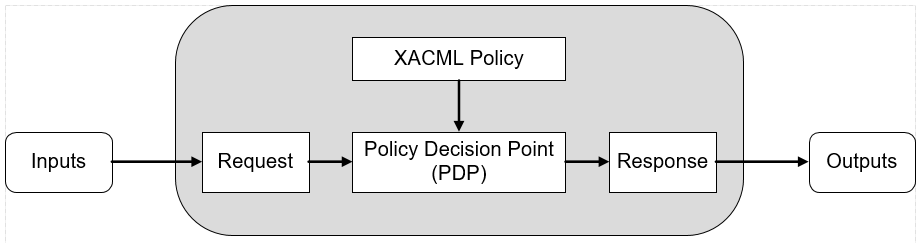
\includegraphics[width=.95\textwidth]{xacml-context}
    \caption{The context diagram of \acrshort{xacml}. From~\cite{OASISStandard2013EXtensible3.0}, edited.
    }
    \label{fig:xacml-context}
\end{figure}
 
The \acrshort{xacml} standard defines in detail several logical entities and their interactions. The native format for messages between these entities is XML, but a profile has been developed to support JSON message format~\cite{2017JSON1.0}. Additional profile was also created to describe implementation in a RESTful architecture~\cite{2017REST1.0}.
 
 Several implementations of \acrshort{xacml} exist in Java, Python and other languages. Criticisms of \acrshort{xacml} include low adoption rate, unsuitability for federated enterprises~\cite{Cser2013XACMLDead}, and lack of transparency for the end user~\cite{Cser2013XACMLDead, Ardagna2011ExpressiveApplications}.


\subsection{SAML}\label{sec:saml}

The \acrfull{saml} is a framework for exchange of assertions containing security information between two online parties, typically an identity provider and a relying party. Similarly as XACML, \acrshort{saml} was developed by OASIS. Version 1.0 was released in 2002 and version 2.0 (latest) in 2005. The rest of this report refers to version 2.0.

The main premise of \acrshort{saml} is that the \acrfull{idp} and the protected resource/application are two separated entities. This is desired, since it enables us to manage identities centrally for multiple applications and avoids duplication user accounts across these applications. Moreover, separating these enables both parts to specialise only in their task.

The Figure~\ref{fig:saml-architectire} illustrates the separation of these two entities. It also depicts the high-level flow of the authentication process. If the user wants to access the protected resource on the right, they first need to authenticate themselves with the \acrshort{idp}.

Another noteworthy aspect of \acrshort{saml} is the identity federation. This is achieved, when the \acrshort{idp} and the \acrshort{rp} are in different security realms, possibly operated by different organisations. As long as an agreement is established between the two, users can use identity managed by the \acrshort{idp} to access any resources outside the organisation's boundary~\cite{2008SecurityOverview}.

 \begin{figure}[ht]
    \centering
    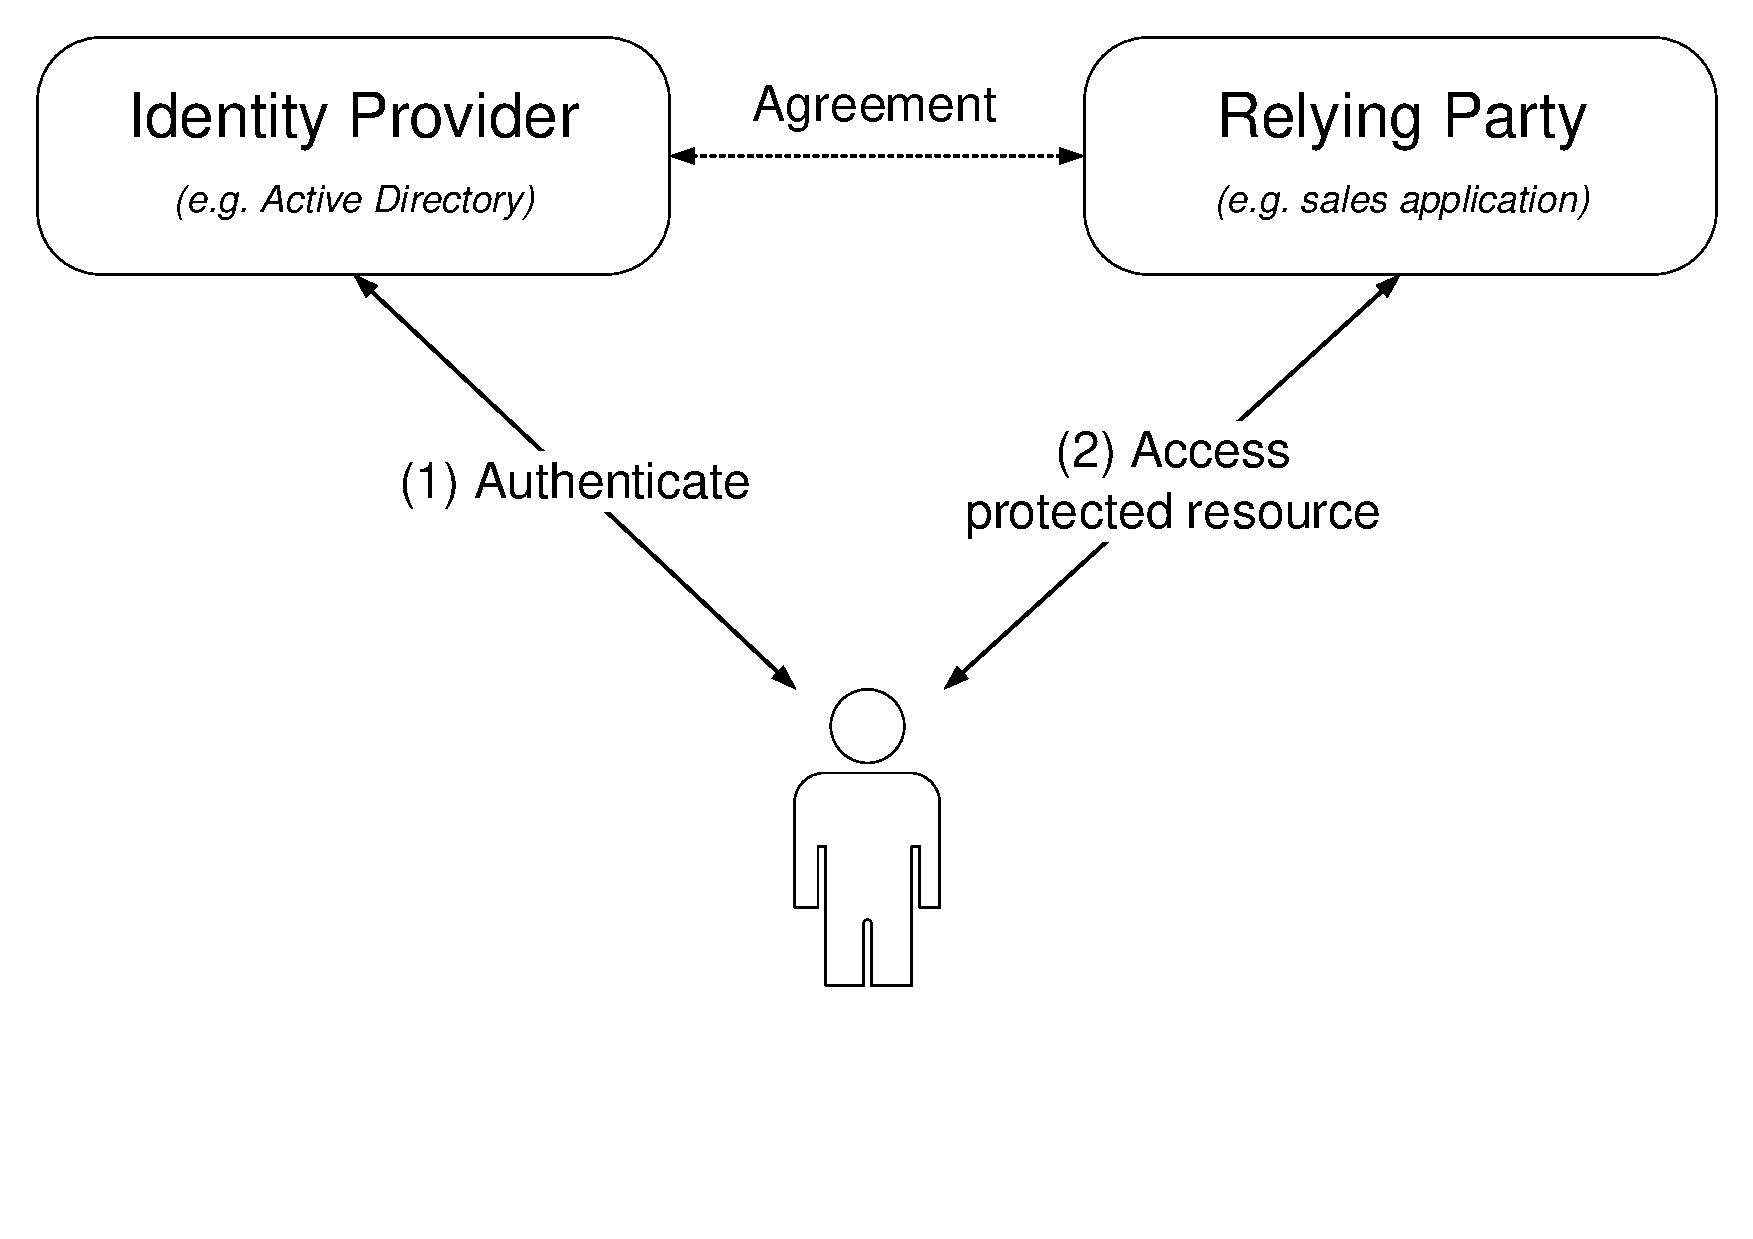
\includegraphics[width=.95\textwidth]{saml-architecture}
    \caption{The general use case of SAML, demonstrating the premise of functional separation of \acrshort{idp} and \acrshort{rp}. Taken from~\cite{2008SecurityOverview}.}
    \label{fig:saml-architectire}
\end{figure}

\paragraph{Assertions}
An assertion in \acrshort{saml} contains some security information about the \textit{subject}. Subject could be the user Bob and the associated information could be Bob's email address and job title. The security information need to be of one of following three categories:

\begin{enumerate*}[label=(\roman*)]
    \item \textit{Authentication statements} describe means and the timestamp of the authorisation carried out by the asserting party;
    \item \textit{Attribute statements} provide information about the subject; and
    \item \textit{Authorisation decision statement} describes what the subject is permitted to access in the system.
\end{enumerate*}

% \paragraph{Protocols}
% \acrshort{saml} defines a number of general protocols to facilitate the message exchange during different parts of the assertion process.

\paragraph{Bindings}
\acrshort{saml} describes how the messages exchanged during an assertion process can be bound to lower-level transport protocols. There are in total 6 bindings defined by the standard, but the following three are of particular interest:

\begin{itemize}[noitemsep]
    \item \textit{HTTP Redirect Binding}, where the entire \acrshort{saml} message is carried in the URL parameters, in the header of an HTTP GET method. This is suitable for short messages as the length of URL is limited in practice. This binding can be used in a RESTful system.
    \item \textit{HTTP POST Binding}, where the \acrshort{saml} message is base64 encoded into an XHTML form and transmitted using the HTTP POST method. This binding can also be used in a RESTful system.
    \item \textit{SAML SOAP Binding} specifies how the \acrshort{saml} messages are carried in an XML envelope over SOAP over any underlying transport protocol~\cite{Cantor2005BindingsV2.0}.
\end{itemize}

% \paragraph{Profiles}
% Several profiles which build on assertions and bindings are defined in the standard which correspond to the most common use cases of \acrshort{saml}. 

While \acrshort{saml} is widely adopted in the industry and is considered generally secure, numerous security flaws have been identified over time. Most of these arised from improper implementation of the protocol and have been patched since discovery~\cite{Krawczyk2014SecureAttacks}. The vulnerabilities included XML signature wrapping, assertion eavesdropping~\cite{Chen2014Environment-BoundAssertions} and XML parsing issues~\cite{Degges2018AVulnerability}.
\subsection{NIST Digital Identity Guidelines}

The \acrfull{nist} developed a set of guidelines, intended primarily to govern how public authorities in the US implement digital authentication in non-national-security scenarios. Yet, it was adopted by by wider community, spanning out of the government sector.
% REFERENCE Government Adopts an Industry Approach to Open Source Collaboration

The guidelines contain three volumes, covering three distinct areas of authentication:
\begin{enumerate*}[label=(\roman*)]
    \item SP 800-63A focused on Enrolment and Identity Proofing;
    \item SP 800-63B centred around Authentication and Lifecycle Management; and
    \item SP 800-63C covering federation and assertions.
\end{enumerate*}
The guidelines advertise the use of authentication to mitigate risks of unauthorised access to protected resources, but also promote minimising the collection of \acrfull{pii} and use of pseudonymous information whenever possible.
%REFERENCE Digital identity guidelines: revision 3

The guidelines define a Digital Identity Model (Figure~\ref{fig:nist-model}), which is useful to distinguish the various types of roles and activities within an authentication system. On the left side of the model there is a \acrfull{csp}. \acrshort{csp} is an entity that issues electronic credentials and registers user's \textit{authenticator} (authenticator is something that the user has or controls). On the right side of the model is the verifier, whose task is to authenticate users by validating binding of their authenticators to their credentials.
% %REFERENCE Digital identity guidelines: revision 3

 \begin{figure}[ht]
    \centering
    % TODO Change figure in visio
    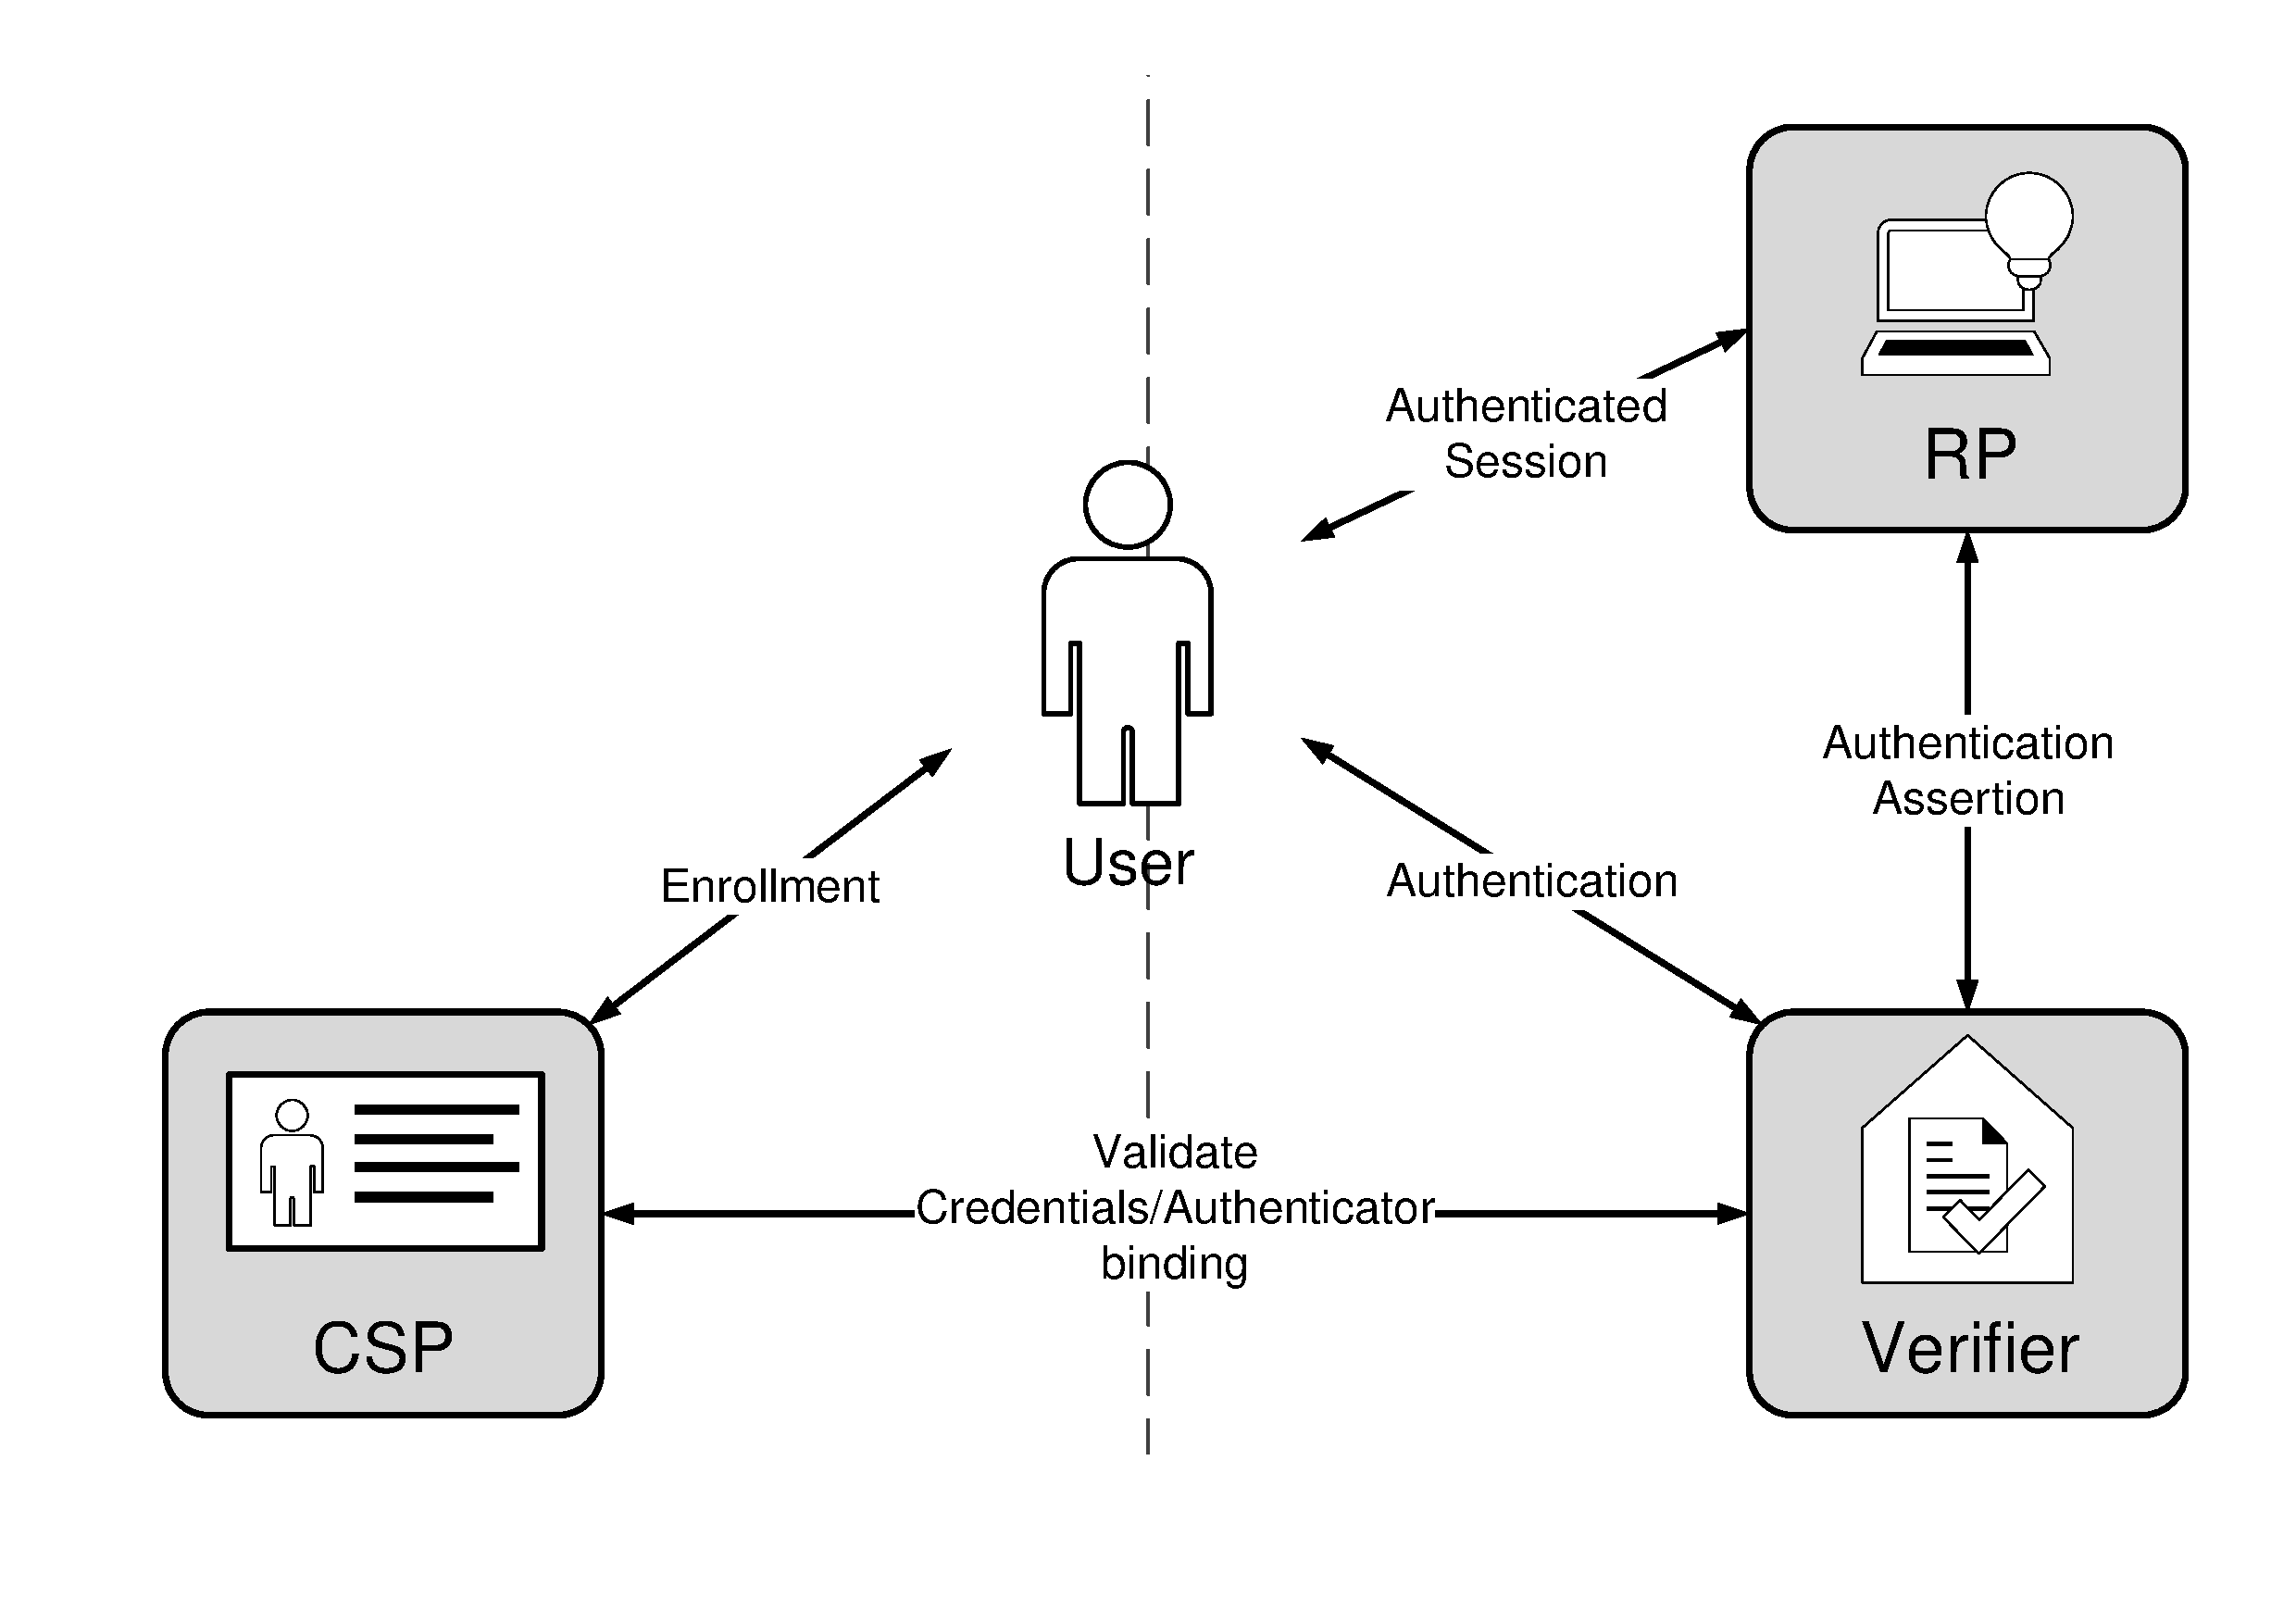
\includegraphics[width=.95\textwidth]{nist-simplified}
    \caption{Digital Identity Model (simplified). The left side of the figure represents enrolment of the user with the \acrshort{csp}. The right part of the user represents authentication with the verifier, before an authenticated session is established between the user and the \acrshort{rp}. Taken from (edited).
    % %REFERENCE Digital identity guidelines: revision 3
    }
    \label{fig:nist-model}
\end{figure}

\paragraph{SP 800-63A}
This volume of the Digital Identity Guidelines defines three Identity Assurance Levels (IALs) and requirements on identity proofing for each level. The \acrshort{ial}1 requires no verification of assertions provided by the user. \acrshort{ial}2 requires either remote or physically-present verification of assertions made by the user, while \acrshort{ial}3 requires manual verification by a trained person, representing the \acrshort{csp}.

% REFERENCE Digital identity guidelines: enrollment and identity proofing

\paragraph{SP 800-63B}
The B volume of the Guidelines defines three Authenticator Assurance Levels (AALs).

To authenticate themselves in AAL1, the user needs to demonstrate control of one authenticator. This must be done through a secure authentication protocol.

In AAL2, the user must demonstrate control of two distinct authenticators. This can be in a form of a multi-factor authenticator, or single-factor possession-based authenticator together with a memorised password. Cryptographic techniques defined in
% REFERENCE SECURITY REQUIREMENTS FOR CRYPTOGRAPHIC MODULES
must be used.

In AAL3, a hardware-based authenticator must be used in addition to requirements of AAL2. Furthermore, one of the authenticators used must be resistant to attacks attempting to impersonate the user.

\paragraph{SP 800-63C}
The C volume of the guidelines describes the use of assertions for identity federation across several \acrshort{rp}s. This enables the user to use services provided by several \acrshort{rp}s, while maintaining only a single identity at one \acrshort{idp}. The volume also describes three Federation Assurance Levels, however we do not cover these in this report.
% REFERENCE Digital identity guidelines: federation and assertions

\paragraph{Authenticator types}

% TODO WRITE HERE
\subsection{OAuth 2.0} \label{sec:OAuth_2}

Before existence of OAuth, the access to user's protected resources was commonly delegated to a third party by sharing the user's credentials with that third party. This approach has flaws, since it is not possible for the user to fine-tune the access to their account, neither across different third parties, nor for different access levels of any given third party. 

The OAuth 1.0 was published in 2010 as to address this problem~\cite{Hammer-Lahav2010TheProtocol} and was followed in 2012 by OAuth 2.0~\cite{Hardt2012TheFramework}. OAuth 2.0 is not compatible with version 1.0 and is widely used today. In the following sections of this report we will refer to OAuth 2.0.

Using the OAuth framework, a third-party application may obtain a fine-grained access to protected resources. The third-party application requesting access to user's protected resources is known as the \textit{client}. The server controlling the protected resources has an authorisation server associated with it. The standard defines four distinct ways (called \textit{grant types}, how the client can obtain the access by communicating with the authorisation server. Before we describe these grant types, let us first draw the difference between different clients.

\paragraph{Client types} OAuth distinguishes three client types:
\begin{itemize}[noitemsep]
    \item \textit{Web-based application} is an application that runs on a web server and communicates with the user over HTML via a browser. Web-based application is considered secure, as the user and application secrets can be stored on the web server.
    \item \textit{User-agent-based application} is downloaded from the server, but afterwards runs on the user's device. This is considered less secure than web-based application, as any secrets could be potentially exposed by the user-agent (browser).
    \item \textit{Native application} is installed by the user and runs directly on user's device. It can offer good protection to secrets entered by the user during runtime, but any application secrets which are included and shipped with the application could be potentially exposed~\cite{Hardt2012TheFramework}.
\end{itemize}

\paragraph{Grant types} Four grant types are defined by the standard. Not all grant types are suitable for all client types, but other parameters, such as desired level of security or preference are also parameters for the choice of the grant type. The defined types are as follows:

\begin{itemize}[noitemsep]
    \item \textit{Authorisation Code Grant}. Using this grant type, the user is first directed from the web-based application to authenticate with the authorisation server. After user authenticates, they they are asked by the authorisation server to give consent for the client application to use the protected resources controlled by the user. Once the consent is given, the user agent receives an authorisation code from the authentication server. This authorisation code is passed to the web server via HTTP redirect method. The client running on the web server contacts the authorisation server with the authorisation code to obtain an access token. The access token is presented when the client application accesses the protected resource. This flow is illustrated in Figure~\ref{fig:oauth-code-grant}.
    \item \textit{Implicit Grant}. In this grant type, the client application is typically running in the user agent. The flow is similar to the one described above, but instead of the authorisation code, the access token is sent directly to the client application. This is simpler than the authorisation code grant, but less secure, since the access token can be captured by other applications residing on the user's device.
    \item \textit{Resource Owner Password Credentials Grant}. When using this grant type, user's credentials need to be shared directly with the client application. This is only suitable, if the client application is fully trusted by the user.
    \item \textit{Client Credentials Grant} is used when the client application requires access to own resources (as opposed to user's protected resources).
\end{itemize}

\begin{figure}[ht]
    \centering
    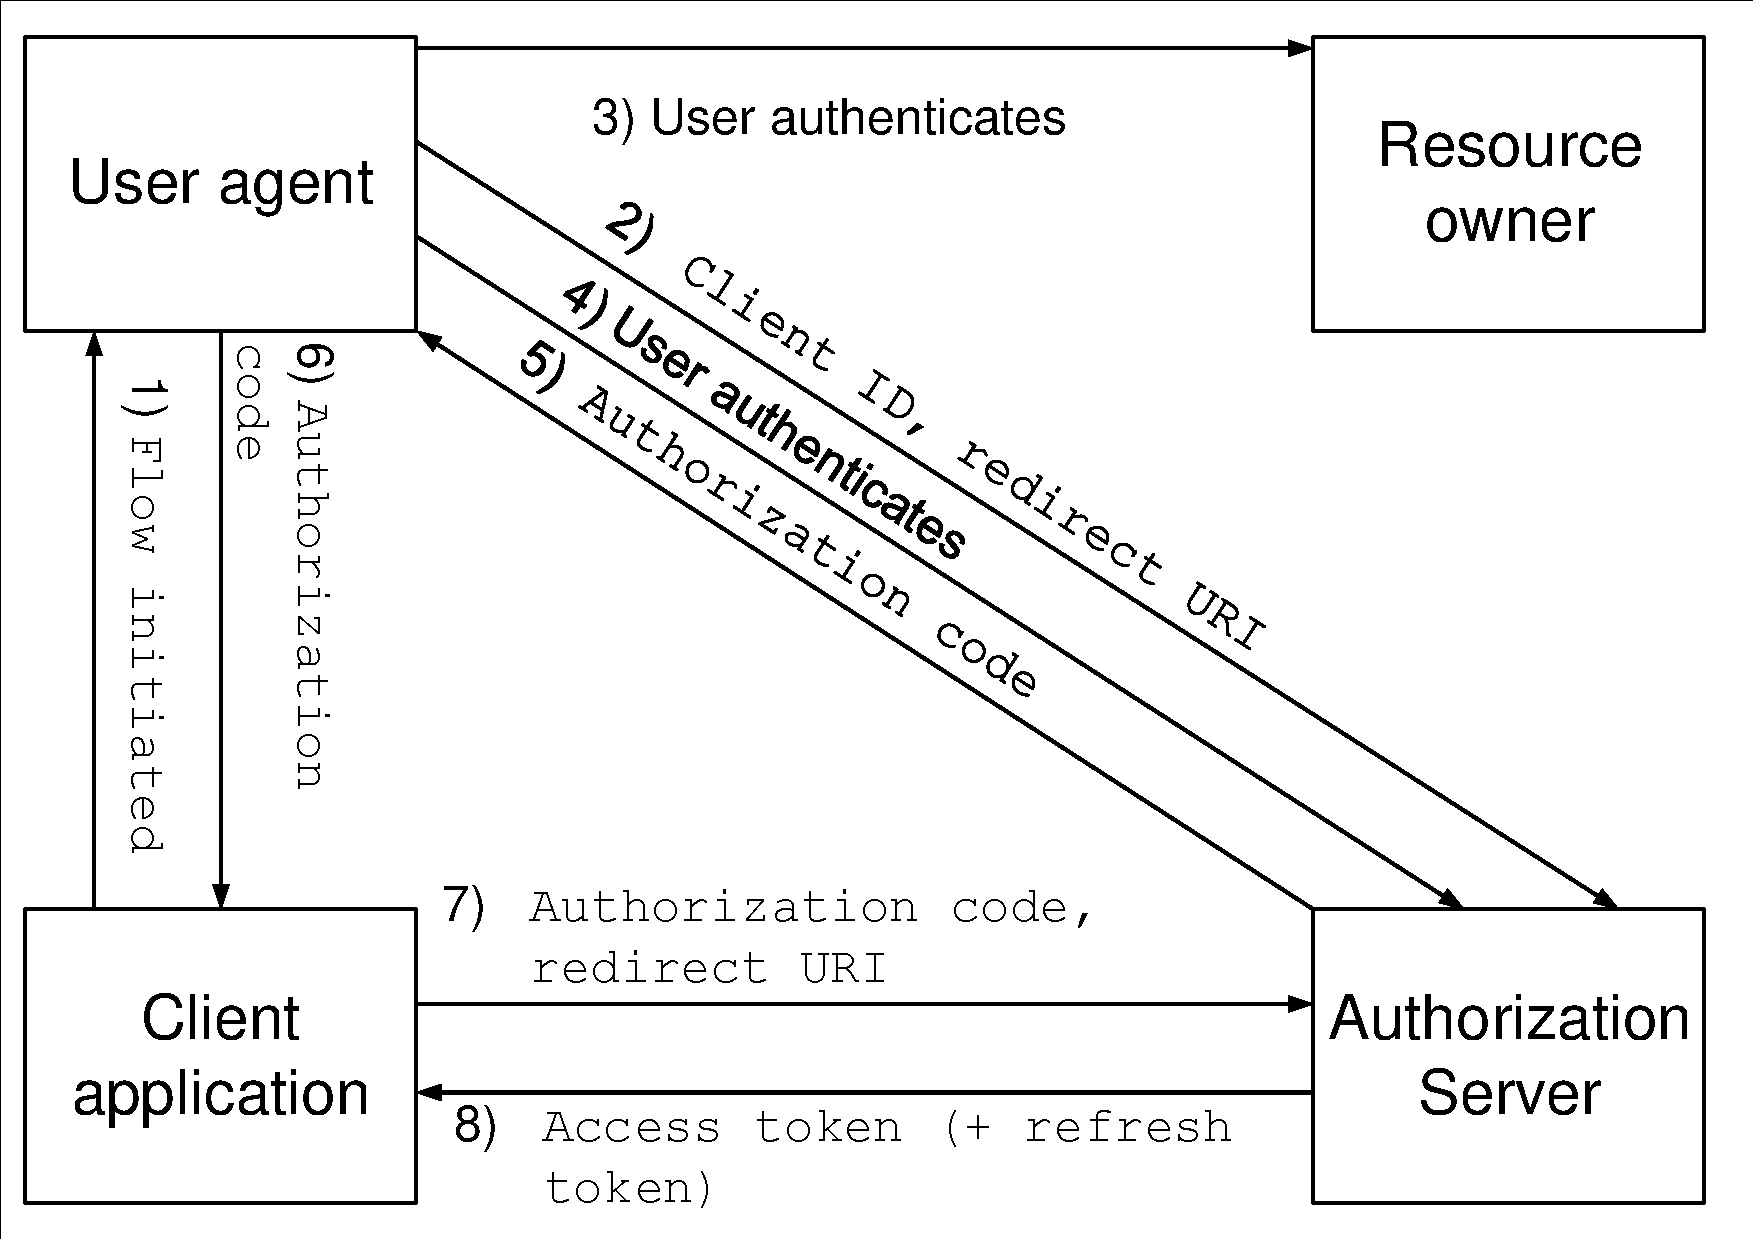
\includegraphics[width=.95\textwidth]{oauth-code-grant}
    \caption{OAuth Authorisation code grant. The user authenticates with the authorisation server and gives consent for access to their protected resources. An authorisation code is sent to the redirect URI specified in the original request. This access token is forwarded to the web server hosing the client application and exchanged for an access token at the authorisation server. From~\cite{Hardt2012TheFramework}, edited.}
    \label{fig:oauth-code-grant}
\end{figure}

\paragraph{Access token scopes}
Scope in the OAuth context typically represents a piece of functionality or data, access to which can be individually controlled. Well defined scopes allow for granular access control. The client application includes the \textit{scope} parameter in the authorisation request to inform the authorisation server, which data or functionality it wishes to access. The authorisation server may grant access to any number of the requested scopes, based on the internal policy and user's consent~\cite{Hardt2012TheFramework}.

The process outlined above is mostly concerned with authorisation of the client to access protected resources. However, it emerged as a common, albeit incorrect practice that OAuth was used to authenticate users~\cite{RicherUser2.0}, by allowing the client to only read a scope that contains the basic user data. While it is technically possible to achieve this using OAuth alone, further specifications were developed to standardise this usecase. We cover these in the following section.
% FINAL check if following section is about OpenID Connect